\chapter{Ecología del comportamiento}\label{ch:b3:behavioural-ecology}

Un suricata se yergue sobre un termitero mientras el resto de su grupo
escarba en busca de comida y, cuando aparece un halcón, ladra y los
demás corren a sus madrigueras. El centinela ha pasado una hora sin
comer y se ha convertido en el animal más llamativo del desierto. ¿Por
qué? Un pavo real arrastra una cola que le cuesta la quinta parte de su
presupuesto energético y le frena la huida de los tigres. Una abeja que
vuelve de un campo baila sobre un panal vertical, y el ángulo de su
danza respecto de la vertical es el ángulo del alimento respecto del
sol. Un carbonero que caza orugas en un rodal de follaje lo abandona
cuando todavía quedan orugas por encontrar. Ninguno de estos animales ha
leído este capítulo y, sin embargo, cada uno se comporta como si hubiera
resuelto una optimización, un juego o un problema de contabilidad de
parentesco. La ecología del comportamiento es el estudio de la conducta
como un conjunto de soluciones evolucionadas: para qué sirve una
conducta, en términos de los genes que propaga, y cuáles han de ser sus
costes y sus beneficios para que la selección natural la haya producido.
Sus herramientas son las que usa un economista ---la optimización, la
\omterm{prop:b3:behavioural-ecology:hawk-dove}{teoría de juegos}, la contabilidad del parentesco--- y su prueba es el
campo.

\section{Cuatro preguntas y la maquinaria del instinto}

\begin{definition}[Las preguntas de Tinbergen]\label{def:b3:behavioural-ecology:tinbergen}
\index{cuatro preguntas de Tinbergen}\index{pauta fija de acción}\index{estímulo señal}\index{impronta}\index{período crítico}
Tinbergen (1963) dijo que una explicación completa de cualquier
conducta ha de responder a cuatro preguntas: su \emph{mecanismo} (qué
estímulos y qué maquinaria neural la producen), su \emph{desarrollo}
(cómo surge en el individuo, a partir de los genes y de la
experiencia), su \emph{función} (cómo contribuye a la supervivencia y a
la reproducción) y su \emph{historia evolutiva} (cómo surgió de una
conducta ancestral). Los etólogos que las formularon habían establecido
las dos primeras. Muchas conductas son \emph{pautas fijas de acción}:
secuencias estereotipadas que desencadena un simple \emph{estímulo
señal} y que se ejecutan hasta el final una vez comenzadas ---un ánsar
común devuelve al nido con el pico un huevo desplazado y completa el
movimiento aunque se le retire el huevo a medio camino; un pollo de
gaviota argéntea picotea una mancha roja de cualquier objeto con forma
de pico, y picotea más un palo con tres bandas rojas que la cabeza de
una gaviota de verdad; un espinoso macho ataca cualquier cosa roja por
debajo, incluida una furgoneta de correos que pasa vista por la
ventana. Otras se aprenden dentro de una ventana: la \emph{impronta},
por la cual un ansarón, en su primer día, sigue y trata en adelante
como progenitor a lo que se mueva ---un ganso, Lorenz, una caja de
cartón---, es rápida, irreversible y está confinada a un
\emph{período crítico}; el aprendizaje del canto en las aves, el ejemplo
del volumen del Año~2, tiene la misma forma. La dicotomía entre lo
innato y lo aprendido es falsa: una conducta tiene un programa genético
que especifica qué ha de aprenderse, cuándo y de quién, y el programa
es lo que evoluciona.
\end{definition}

\begin{proof}[Evidencia]
Los experimentos de campo de Tinbergen fijaron el método. Las avispas
cavadoras (\emph{Philanthus}) vuelven a un nido escondido en la arena;
él desplazó un anillo de piñas que había colocado alrededor de una
entrada mientras la avispa estaba fuera, y ella buscó en el centro del
anillo desplazado ---había aprendido las referencias. Las gaviotas
reidoras retiran del nido las cáscaras de huevo tras la eclosión; él
dispuso huevos junto a cáscaras pintadas, cáscaras naturales y otros
objetos y contó cuáles se llevaban las cornejas: la superficie interior
blanca de una cáscara atraía a los depredadores, y la retirada que
había parecido pulcritud era camuflaje. Los experimentos con pollos de
gaviota cuantificaron un \omterm{def:b3:behavioural-ecology:tinbergen}{estímulo señal} ofreciendo cabezas de cartón
que variaban un rasgo cada vez. Los gansos improntados de Lorenz lo
siguieron toda la vida; los patos improntados el primer día sobre una
caja en movimiento ya no pudieron hacerse seguir a un pato.
\end{proof}

\begin{omfigure}
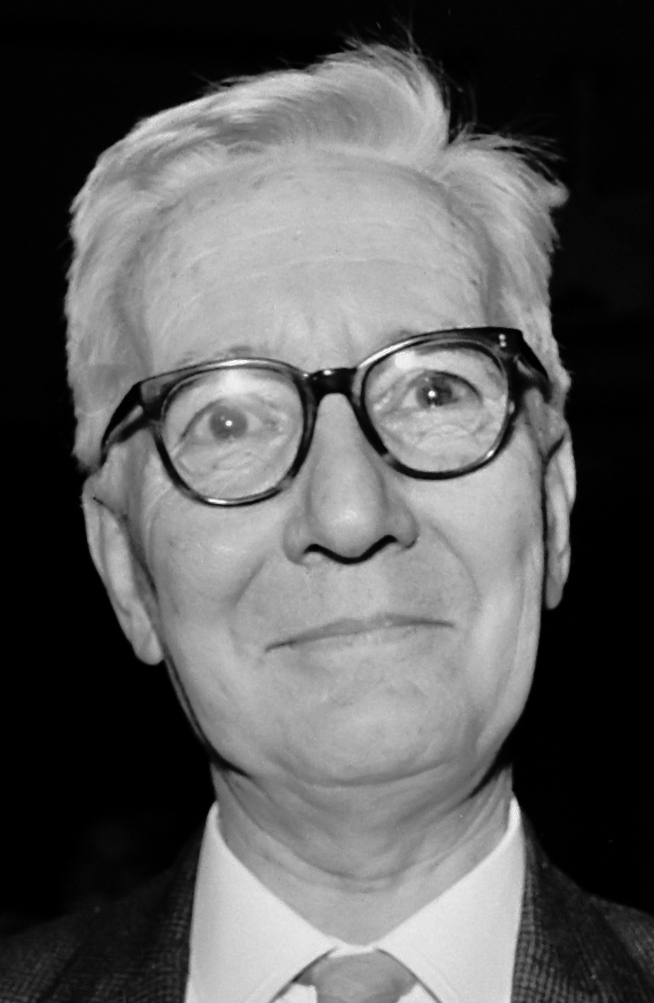
\includegraphics[width=0.36\linewidth]{images/book5/tinbergen.jpg}\hspace{0.04\linewidth}
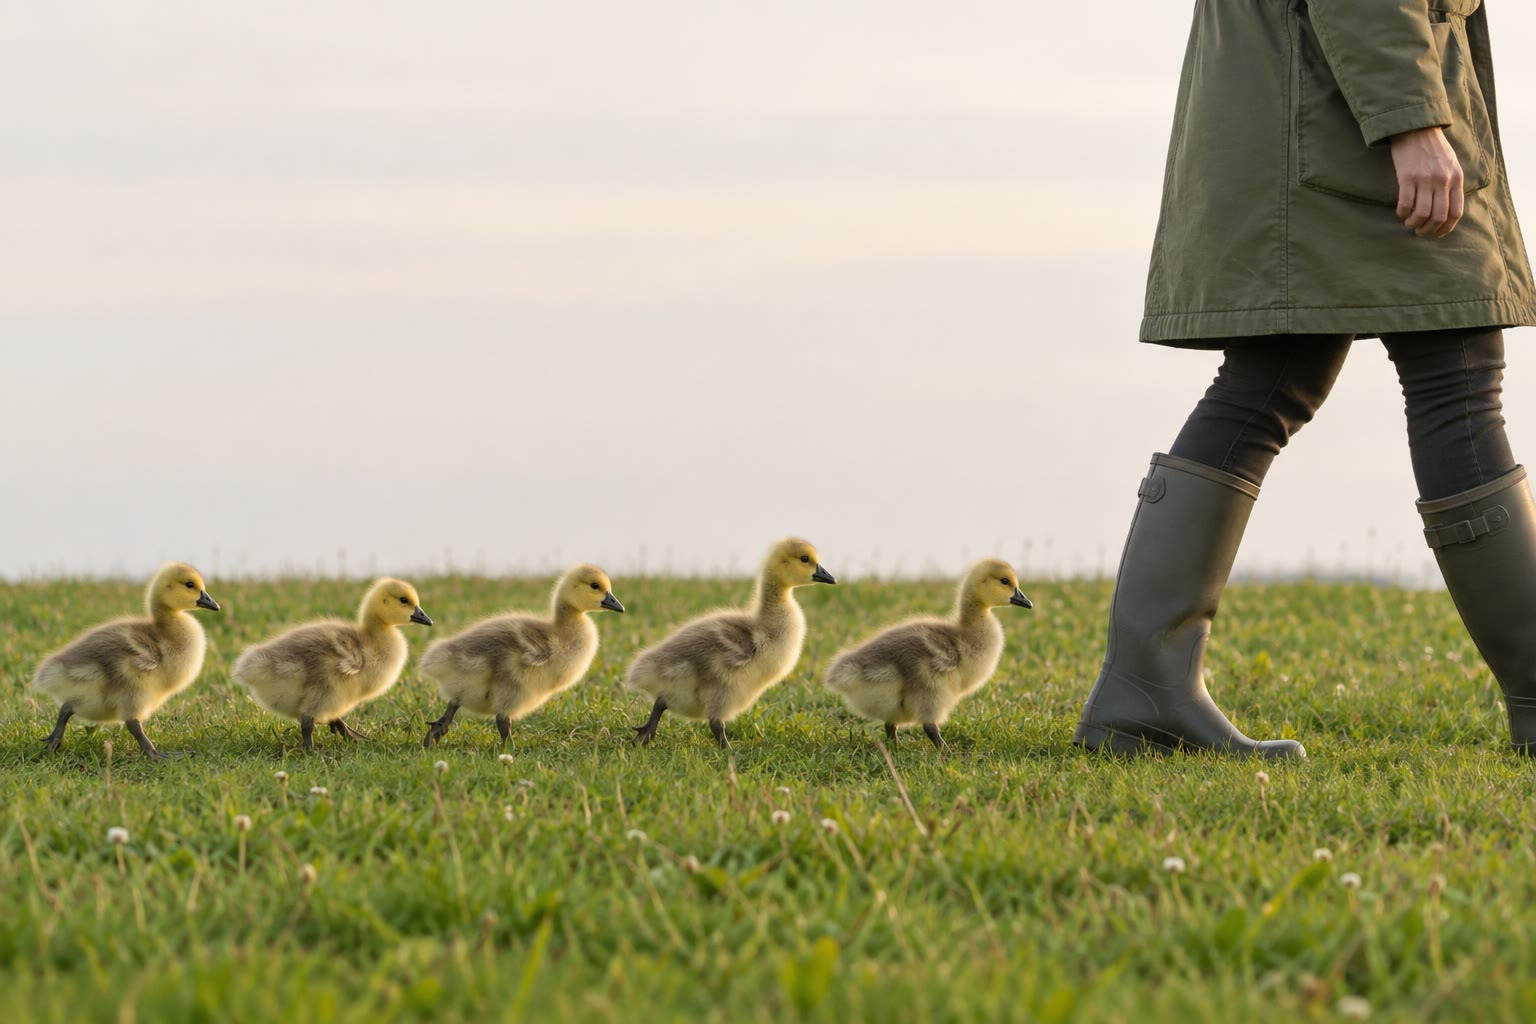
\includegraphics[width=0.52\linewidth]{images/book5/ai/b5-26-goose-imprinting.jpg}

{\small Izquierda: Niko Tinbergen (1907--1988), que llevó las preguntas
de la conducta al campo y las hizo experimentales (fotografía de Rob
Mieremet, Anefo, 1973, CC0). Derecha: ansarones que siguen a la primera
cosa grande en movimiento que vieron, un día después de eclosionar, y a
los que nunca después se convenció de otra cosa.}
\end{omfigure}

\section{Decidir: el forrajeo óptimo}

\begin{theorem}[El teorema del valor marginal]\label{thm:b3:behavioural-ecology:mvt}
\index{forrajeo óptimo}\index{teorema del valor marginal}\index{tiempo de permanencia en el rodal}\index{moneda}
Un forrajeador visita rodales de alimento separados por un tiempo de
viaje $\tau$. En un rodal gana una energía $g(t)$ tras un tiempo $t$,
con $g$ creciente y cóncava (el rodal se agota). Si abandona todos los
rodales tras un tiempo $t$, su ritmo de ganancia a largo plazo es
$R(t) = g(t)/(\tau + t)$, y el tiempo de permanencia $t^{*}$ que lo
maximiza cumple
\[
g'(t^{*}) = \frac{g(t^{*})}{\tau + t^{*}} = R(t^{*}) :
\]
abandónese un rodal cuando el ritmo instantáneo de ganancia en él haya
caído al ritmo medio de todo el hábitat, viaje incluido (Charnov,
1976). Consecuencias: cuanto mayor es el tiempo de viaje, más larga es
la estancia y más a fondo se agota cada rodal; en un hábitat más rico
($R$ mayor) todos los rodales se abandonan antes y menos agotados; y
todos los rodales se abandonan al mismo ritmo marginal, sea cual sea su
calidad, de modo que un rodal pobre se abandona casi de inmediato y uno
rico solo cuando se ha rebajado hasta la media del hábitat. Para
$g(t) = A(1 -
\mathrm{e}^{-t/T_{0}})$ la condición se vuelve $(\tau + t^{*})/T_{0} =
\mathrm{e}^{t^{*}/T_{0}} - 1$, resuelta numéricamente: con $\tau = T_{0}$,
$t^{*} \approx 1.15\,T_{0}$; con $\tau = 4T_{0}$, $t^{*} \approx
2.0\,T_{0}$.
\end{theorem}
\begin{proof}
$R(t) = g(t)/(\tau + t)$; $R'(t) = [g'(t)(\tau + t) - g(t)]/(\tau +
t)^{2} = 0$ da $g'(t^{*}) = g(t^{*})/(\tau + t^{*})$. Geométricamente:
dibújese $g$ frente a $t$ con el origen en $-\tau$; $R(t)$ es la
pendiente de la recta que va de $(-\tau, 0)$ a $(t, g(t))$, máxima allí
donde esa recta es tangente a la curva ---que es la condición. Un
$\tau$ mayor mueve el origen a la izquierda y el punto de tangencia a
la derecha; un hábitat más rico empina la tangente y la mueve a la
izquierda. Para la exponencial, $g' = (A/T_{0})
\mathrm{e}^{-t/T_{0}}$ y $g/(\tau + t) = A(1 - \mathrm{e}^{-t/T_{0}})/
(\tau + t)$; igualando y reordenando se obtiene la ecuación enunciada, y
sustituyendo $t^{*} = 1.15T_{0}$ con $\tau = T_{0}$: a la izquierda
$2.15$, a la derecha $\mathrm{e}^{1.15} - 1 = 2.16$.
\end{proof}

\begin{omfigure}
\begin{tikzpicture}
\begin{axis}[
  width=0.68\linewidth, height=5.8cm,
  axis x line=middle, axis y line=left,
  xmin=-4.5, xmax=5, ymin=0, ymax=1.15,
  xlabel={tiempo (unidades de $T_{0}$)}, ylabel={energía ganada en el rodal},
  xlabel style={font=\small, at={(axis description cs:0.95,0.0)}, anchor=north}, ylabel style={font=\small},
  tick label style={font=\small}, xtick={-4,-1,0,1.15,2}, xticklabels={$-4T_0$,$-T_0$,0,$1.15$,$2.0$}, ytick={0.5,1}, yticklabels={$0.5A$,$A$},
  clip=false,
]
\addplot[very thick, omDef, domain=0:5, samples=80] {1-exp(-x)};
\draw[thick, omThm] (axis cs:-1,0) -- (axis cs:1.55,1.13);
\draw[thick, omMeth!70!black] (axis cs:-4,0) -- (axis cs:3.5,1.081);
\fill[omThm] (axis cs:1.15,0.6834) circle (2pt); \fill[omMeth!70!black] (axis cs:2,0.8647) circle (2pt);
\draw[dashed, gray] (axis cs:1.15,0) -- (axis cs:1.15,0.6834); \draw[dashed, gray] (axis cs:2,0) -- (axis cs:2,0.8647);
\node[font=\scriptsize, omThm, anchor=north west, align=left] at (axis cs:-4.4,1.1) {viaje corto, $\tau = T_{0}$:\\se abandona en $t^{*} = 1.15\,T_{0}$,\\rodal agotado al \qty{68}{\%}};
\node[font=\scriptsize, omMeth!70!black, anchor=north west, align=left] at (axis cs:2.4,0.62) {viaje largo, $\tau = 4T_{0}$:\\se abandona en $t^{*} = 2.0\,T_{0}$,\\agotado al \qty{86}{\%}};
\node[font=\scriptsize, omDef, anchor=north west] at (axis cs:3.0,0.86) {$g(t) = A(1 - \mathrm{e}^{-t/T_{0}})$};
\node[font=\scriptsize, gray, anchor=south] at (axis cs:-2.5,0.02) {viaje};
\end{axis}
\end{tikzpicture}

{\small El \omterm{thm:b3:behavioural-ecology:mvt}{teorema del valor marginal} dibujado. La curva de ganancia se
aplana a medida que el rodal se agota; la recta que va del comienzo del
viaje a un punto de la curva tiene una pendiente igual al ritmo global
de ganancia; el mejor momento para marcharse es allí donde esa recta es
tangente. Un viaje más largo mueve el origen a la izquierda y el punto
de tangencia a la derecha.}
\end{omfigure}

\begin{proof}[Evidencia]
Cowie (1977) dejó que unos carboneros cazaran gusanos de la harina
escondidos en vasos llenos de serrín en una pajarera, manipulando el
tiempo de viaje entre vasos con tapas que costaban más o menos quitar;
las aves se quedaban más tiempo en cada vaso cuando el viaje era más
lento, y seguían la predicción del teorema, superándola ligeramente en
la dirección que explica tener en cuenta el coste energético del viaje.
Los estorninos que llevaban larvas de típula a sus polluelos
(Kacelnik, 1984) tomaban cargas mayores de los comederos situados más
lejos, de nuevo como exige la solución que maximiza el ritmo para una
curva de carga. Ninguna de las dos pruebas demuestra que las aves
calculen tangentes; ambas muestran que la selección ha producido reglas
prácticas cuyo resultado se acerca al óptimo.
\end{proof}

\section{Enfrentamientos: la teoría de juegos}

\begin{proposition}[Halcón--Paloma y la estrategia evolutivamente estable]\label{prop:b3:behavioural-ecology:hawk-dove}
\index{teoría de juegos}\index{juego Halcón--Paloma}\index{estrategia evolutivamente estable}\index{selección dependiente de la frecuencia}
Cuando la mejor conducta depende de lo que hagan los demás no hay
óptimo, sino solo un \emph{juego}. Dos animales se disputan un recurso
que vale $V$; un \emph{Halcón} pelea hasta resultar herido (coste $C$) o
vencedor, y una \emph{Paloma} exhibe y se retira si la atacan. Los pagos
medios son
\[
\begin{array}{c|cc}
 & \text{contra Halcón} & \text{contra Paloma}\\ \hline
\text{Halcón} & (V - C)/2 & V\\
\text{Paloma} & 0 & V/2
\end{array}
\]
Una \emph{\omterm{prop:b3:behavioural-ecology:hawk-dove}{estrategia evolutivamente estable}} (Maynard Smith y Price,
1973) es la que, una vez común, no puede ser invadida por ninguna
alternativa rara. Si $V > C$, Halcón es la EEE: pelear compensa incluso
frente a peleones. Si $V
< C$, ninguna estrategia pura es estable ---una población de Palomas la
invaden los Halcones, que ganan todos los enfrentamientos, y una
población de Halcones la invaden las Palomas, que evitan las heridas---
y la EEE es jugar a Halcón con probabilidad
\[
p^{*} = \frac{V}{C},
\]
o, de forma equivalente, una población en la que esa fracción sean
Halcones. En la EEE las dos estrategias van igual de bien, con una
media de $V(1 -
V/C)/2$ cada una, menos que el $V/2$ que se habría repartido una
población de Palomas: el enfrentamiento cuesta a todos, y nadie puede
hacerlo mejor por su cuenta. La selección es aquí \emph{dependiente de
la frecuencia}: la eficacia de una estrategia cae a medida que se
vuelve común, y por eso los enfrentamientos animales son sobre todo
exhibición y de vez en cuando guerra, y por eso la mezcla persiste.
\end{proposition}
\begin{proof}
Sea $p$ la fracción que juega a Halcón. El pago esperado de un Halcón
es $W_{H} = p(V
- C)/2 + (1 - p)V$; el de una Paloma, $W_{D} = (1 - p)V/2$. $W_{H} - W_{D} =
p(V - C)/2 + (1 - p)V/2 = [V - pC]/2$, positivo para $p < V/C$ y
negativo por encima: los Halcones se extienden cuando son raros y se
podan cuando son comunes, y la frecuencia se asienta donde
$W_{H} = W_{D}$, en $p^{*} = V/C$. Que sea estable se sigue del cambio
de signo: una perturbación de $p$ por encima de $p^{*}$ favorece a las
Palomas y se corrige, y por debajo favorece a los Halcones. Si $V
\ge C$ la diferencia es positiva para todo $p \le 1$ y Halcón se fija.
El pago común en $p^{*}$: $W_{D} = (1 - V/C)V/2$.
\end{proof}

\begin{omfigure}
\begin{tikzpicture}
\begin{axis}[
  width=0.6\linewidth, height=5.4cm,
  axis x line=bottom, axis y line=left,
  xmin=0, xmax=1, ymin=-1, ymax=4.2,
  xlabel={fracción de Halcones $p$}, ylabel={pago esperado},
  xlabel style={font=\small, at={(axis description cs:0.5,-0.12)}, anchor=north}, ylabel style={font=\small},
  tick label style={font=\small}, xtick={0,0.5,1}, xticklabels={0,$p^{*} = V/C$,1}, ytick={0,1,2,4},
  clip=false,
]
\addplot[very thick, omThm, domain=0:1, samples=2] {x*(4-8)/2 + (1-x)*4};
\addplot[very thick, omDef, domain=0:1, samples=2] {(1-x)*4/2};
\draw[dashed, gray] (axis cs:0.5,-1) -- (axis cs:0.5,1);
\fill[black] (axis cs:0.5,1) circle (2pt);
\node[font=\scriptsize, omThm, anchor=north west] at (axis cs:0.5,3.9) {Halcón: $p(V - C)/2 + (1 - p)V$};
\node[font=\scriptsize, omDef, anchor=south west] at (axis cs:0.62,0.9) {Paloma: $(1 - p)V/2$};
\node[font=\scriptsize, anchor=west, align=left] at (axis cs:0.55,2.6) {$V = 4$, $C = 8$:\\EEE en $p^{*} = 0.5$,\\pago $V(1 - V/C)/2 = 1$};
\draw[->, thick, omThm] (axis cs:0.1,-0.5) -- (axis cs:0.4,-0.5); \draw[->, thick, omDef] (axis cs:0.9,-0.5) -- (axis cs:0.6,-0.5);
\node[font=\tiny, anchor=north] at (axis cs:0.25,-0.55) {los Halcones se extienden}; \node[font=\tiny, anchor=north] at (axis cs:0.75,-0.55) {las Palomas se extienden};
\end{axis}
\end{tikzpicture}

{\small El \omterm{prop:b3:behavioural-ecology:hawk-dove}{juego Halcón--Paloma}. Allí donde se cruzan las rectas de
pago, las dos estrategias van igual de bien y ninguna puede
extenderse; a uno y otro lado, la selección devuelve la frecuencia a su
sitio. La mezcla es estable y cuesta a todos, y es el aspecto que
tienen los enfrentamientos animales.}
\end{omfigure}

\begin{example}[Juegos en el campo]\label{ex:b3:behavioural-ecology:games}
Los machos de la mariposa nesóbara se disputan los claros de sol del
suelo del bosque: el residente gana casi siempre un breve vuelo en
espiral, y cuando se engaña a dos machos para que ambos se crean
residentes la pelea dura diez veces más ---una convención (``gana el
residente'') que resuelve los enfrentamientos de forma barata y que es
ella misma una EEE cuando pelear es costoso y el recurso no vale gran
cosa. Los machos de la mosca del estiércol esperan a las hembras sobre
las boñigas y se marchan cuando el ritmo de llegadas cae hasta lo que
ofrecería una boñiga fresca ---de nuevo el \omterm{thm:b3:behavioural-ecology:mvt}{teorema del valor marginal},
en un juego en el que el valor del rodal depende de cuántos rivales se
posen en él. Las avispas de los higos, las lagartijas manchadas con
tres tipos de macho que se vencen cíclicamente como en piedra, papel o
tijera, y los machos ``furtivos'' del salmón y del pez luna, que
fecundan huevos colándose junto a los machos territoriales con los que
no pueden pelear, son todos mezclas mantenidas en frecuencias donde las
alternativas pagan igual. La guerra de desgaste ---dos animales que se
exhiben hasta que uno se rinde, siendo la EEE persistir durante un
tiempo aleatorio extraído de una distribución exponencial--- describe
los duelos de miradas de muchas especies, y predice, correctamente, que
la persistencia del perdedor no delata nada sobre cuánto habría durado.
\end{example}

\section{Los parientes: la regla de Hamilton}

\begin{theorem}[La regla de Hamilton]\label{thm:b3:behavioural-ecology:hamilton}
\index{regla de Hamilton}\index{selección de parentesco}\index{parentesco}\index{eficacia inclusiva}\index{altruismo}\index{haplodiploidía}
Un alelo que hace a su portador realizar un acto que le cuesta $c$
descendientes y da a un pariente $b$ descendientes de más se extiende si
\[
r\,b > c ,
\]
donde $r$ es el \emph{coeficiente de parentesco}: la probabilidad de
que un gen del receptor sea una copia, por descendencia, del mismo gen
del actor ---$1/2$ para progenitor e hijo o para hermanos completos,
$1/4$ para medio hermanos, nietos y sobrinos, y $1/8$ para primos
hermanos. La magnitud que el alelo maximiza es la \emph{\omterm{thm:b3:behavioural-ecology:hamilton}{eficacia
inclusiva}} de su portador: su propia reproducción más sus efectos sobre
la reproducción de sus parientes, ponderada cada una por $r$. El
\emph{altruismo} ---una conducta que baja la reproducción del actor y
sube la de otro--- evoluciona, pues, hacia los parientes, en proporción
al parentesco, y la regla predice dónde debería hallarse: en las
llamadas de alarma de las hembras de las ardillas terrestres, que viven
entre sus hermanas e hijas, y no en las de los machos, que se
dispersan; en la guardia de los suricatas, cuyo grupo es una familia;
en los ayudantes en el nido de las aves que asisten a sus padres en la
cría de hermanos cuando los territorios están llenos. En los
himenópteros \emph{haplodiploides} ---machos a partir de huevos no
fecundados con un solo juego de cromosomas, hembras con dos---, las
hermanas completas comparten tres cuartas partes de sus genes
($r = 3/4$), más de lo que una madre comparte con sus hijas ($1/2$), lo
que Hamilton propuso como razón de que las castas obreras estériles de
hormigas, abejas y avispas surgieran allí once veces y casi en ninguna
otra parte.
\end{theorem}
\begin{proof}
Considérense las copias del alelo. Cuando el actor realiza el acto, sus
propias copias pierden $c$ en transmisión esperada; el receptor lleva el
alelo con una probabilidad $r$ por encima de la media poblacional, de
modo que la ganancia $b$ del receptor aumenta la transmisión del alelo
en $rb$ en promedio. El alelo aumenta en frecuencia cuando $rb - c > 0$
(Hamilton, 1964; la deducción general, a partir de la covarianza entre
el genotipo de un individuo y su eficacia, es la ecuación de Price,
admitida aquí). Parentesco: un progenitor transmite cada gen a un hijo
con probabilidad $1/2$; dos hermanos completos recibieron cada uno un
gen dado del mismo progenitor con probabilidad $1/2$, y es la misma
copia con probabilidad $1/2$, y hay dos progenitores:
$r = 2\times\tfrac{1}{2}
\times\tfrac{1}{2} = \tfrac{1}{2}$. Hermanas haplodiploides: de su padre
haploide reciben genes idénticos (probabilidad $1$); de su madre, copias
idénticas con probabilidad $1/2$; promediando sobre los dos
progenitores, $r = (1 + 1/2)/2 = 3/4$.
\end{proof}

\begin{omfigure}
\begin{tikzpicture}[every node/.style={font=\scriptsize}, >=stealth]
  % diploid pedigree
  \node[draw, circle, fill=omDef!30, minimum size=6mm] (m) at (0,3) {}; \node[draw, fill=omDef!30, minimum size=6mm] (f) at (1.6,3) {};
  \node[above, font=\tiny] at (0.8,3.4) {progenitores diploides};
  \draw[thick] (m) -- (f);
  \node[draw, circle, fill=omThm!40, minimum size=6mm] (a) at (0,1.5) {}; \node[draw, circle, fill=omDef!15, minimum size=6mm] (s) at (1.6,1.5) {};
  \draw[thick] (0.8,3) -- (0.8,2.2) -- (0,2.2) -- (a); \draw[thick] (0.8,2.2) -- (1.6,2.2) -- (s);
  \node[draw, circle, fill=omDef!15, minimum size=6mm] (c) at (1.6,0) {}; \draw[thick] (s) -- (c);
  \node[draw, circle, fill=omDef!15, minimum size=6mm] (o) at (0,0) {}; \draw[thick] (a) -- (o);
  \node[left, omThm, font=\tiny] at (-0.4,1.5) {actor};
  \node[right, font=\tiny] at (1.95,1.5) {hermano completo: $r = 1/2$};
  \node[right, font=\tiny] at (1.95,0) {sobrina: $r = 1/4$};
  \node[left, font=\tiny] at (-0.4,0) {descendencia propia: $1/2$};
  \node[right, font=\tiny] at (1.95,3) {progenitor: $r = 1/2$};
  % haplodiploid
  \begin{scope}[shift={(7.2,0)}]
    \node[draw, circle, fill=omDef!30, minimum size=6mm] (q) at (0,3) {}; \node[draw, fill=omMeth!40, minimum size=6mm] (d) at (1.6,3) {};
    \node[above left, font=\tiny] at (0.1,3.3) {reina (diploide)}; \node[above right, font=\tiny] at (1.5,3.3) {zángano (haploide)};
    \draw[thick] (q) -- (d);
    \node[draw, circle, fill=omThm!40, minimum size=6mm] (w) at (0,1.5) {}; \node[draw, circle, fill=omDef!15, minimum size=6mm] (w2) at (1.6,1.5) {};
    \draw[thick] (0.8,3) -- (0.8,2.2) -- (0,2.2) -- (w); \draw[thick] (0.8,2.2) -- (1.6,2.2) -- (w2);
    \node[left, omThm, font=\tiny] at (-0.4,1.5) {obrera};
    \node[right, align=left, font=\tiny] at (1.95,1.5) {hermana completa: $r = 3/4$\\(los del padre, idénticos;\\los de la madre, con $1/2$)};
    \node[draw, circle, fill=omDef!15, minimum size=6mm] (wd) at (0,0) {}; \draw[thick] (w) -- (wd);
    \node[right, font=\tiny] at (0.35,0) {hija propia: $1/2$: menos que una hermana};
  \end{scope}
  \node[below, align=center] at (4.6,-0.9) {regla de Hamilton: ayúdese cuando $r\,b > c$;\\una obrera haplodiploide que cría hermanas transmite\\más genes propios por descendiente que una que cría hijas};
\end{tikzpicture}

{\small El parentesco en dos clases de familia. En un linaje diploide un
hermano vale media descendencia; en una colonia haplodiploide una
hermana vale más que una hija, lo que inclina la aritmética a quedarse
en casa a ayudar.}
\end{omfigure}

\begin{proof}[Evidencia]
Sherman (1977) observó ardillas terrestres de Belding durante tres
veranos y registró quién daba llamadas de alarma ante los depredadores
que se acercaban: las hembras con parientes cerca llamaban mucho más a
menudo que las hembras sin ellos y que los machos, que se habían
dispersado de su lugar de nacimiento y no tenían parientes al alcance
del oído ---quien llamaba atraía la atención del depredador, y lo
pagaba, solo cuando había parientes a los que avisar. Los abejarucos
frentiblancos de Emlen ayudan en el nido en proporción al parentesco, y
eligen entre los nidos disponibles los de los parientes más próximos.
El estudio a largo plazo de los suricatas de Clutton-Brock halló que
los centinelas eran los individuos bien alimentados, los que menos
tenían que perder, y que la supervivencia del grupo ---y por tanto la
de los parientes del centinela--- subía con el esfuerzo de vigilancia;
el coste, en cambio, resultó menor de lo que suponía el relato, pues un
centinela subido a un montículo suele ser el primero en llegar a una
madriguera.
\end{proof}

\begin{omfigure}
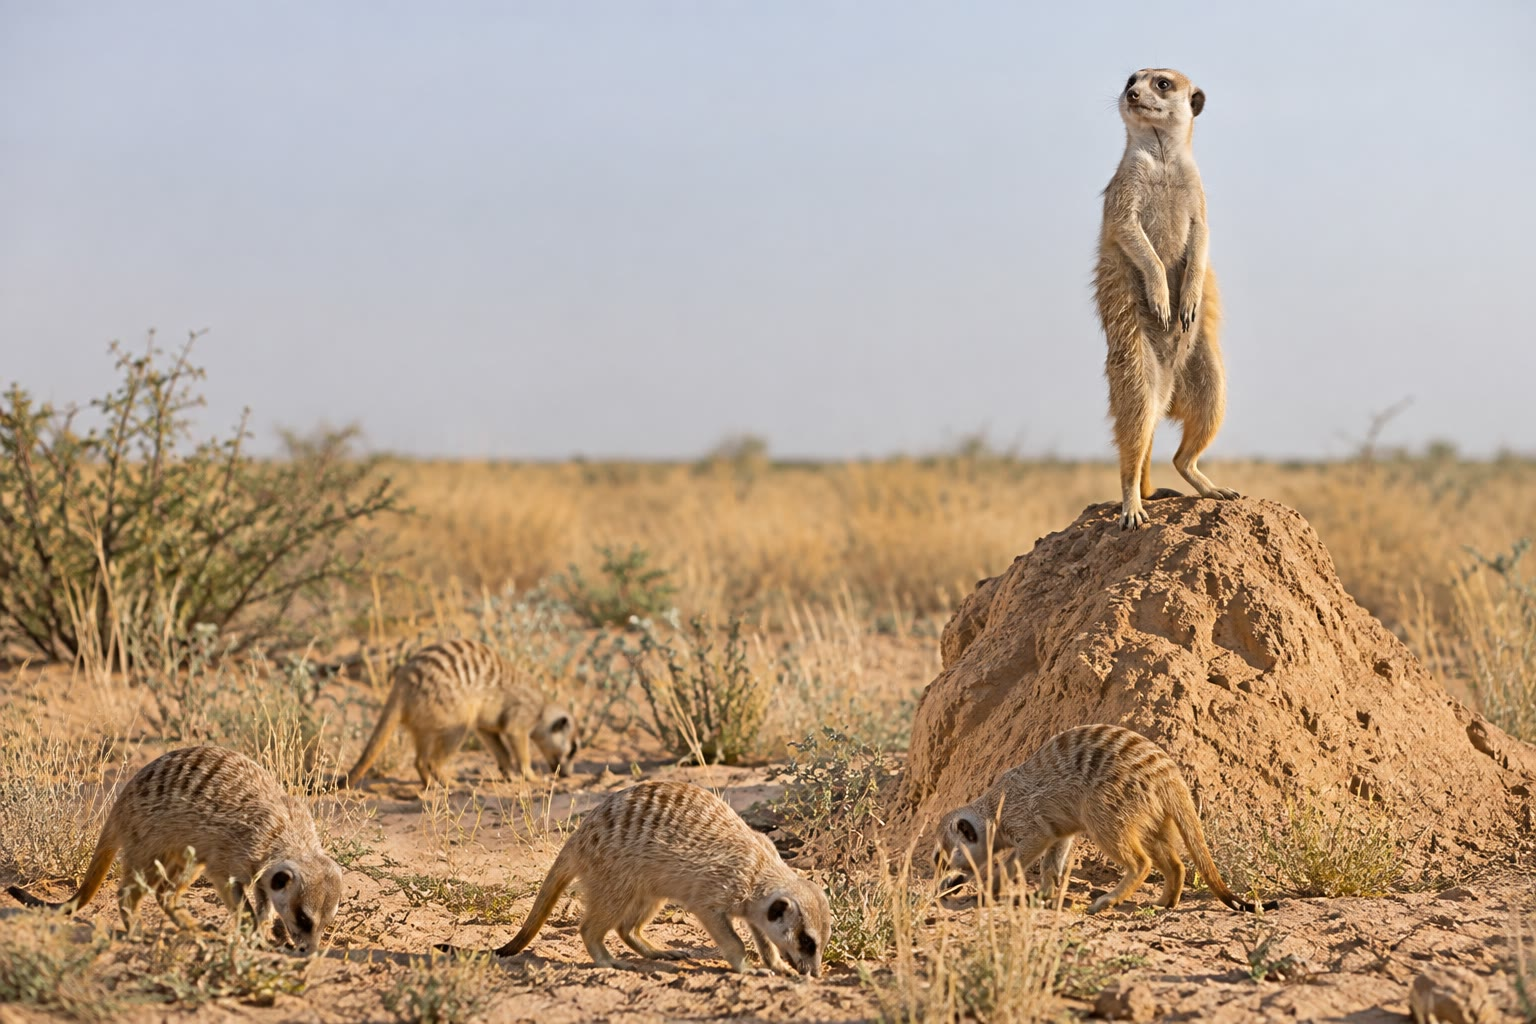
\includegraphics[width=0.46\linewidth]{images/book5/ai/b5-26-meerkat-sentinel.jpg}\hspace{0.04\linewidth}
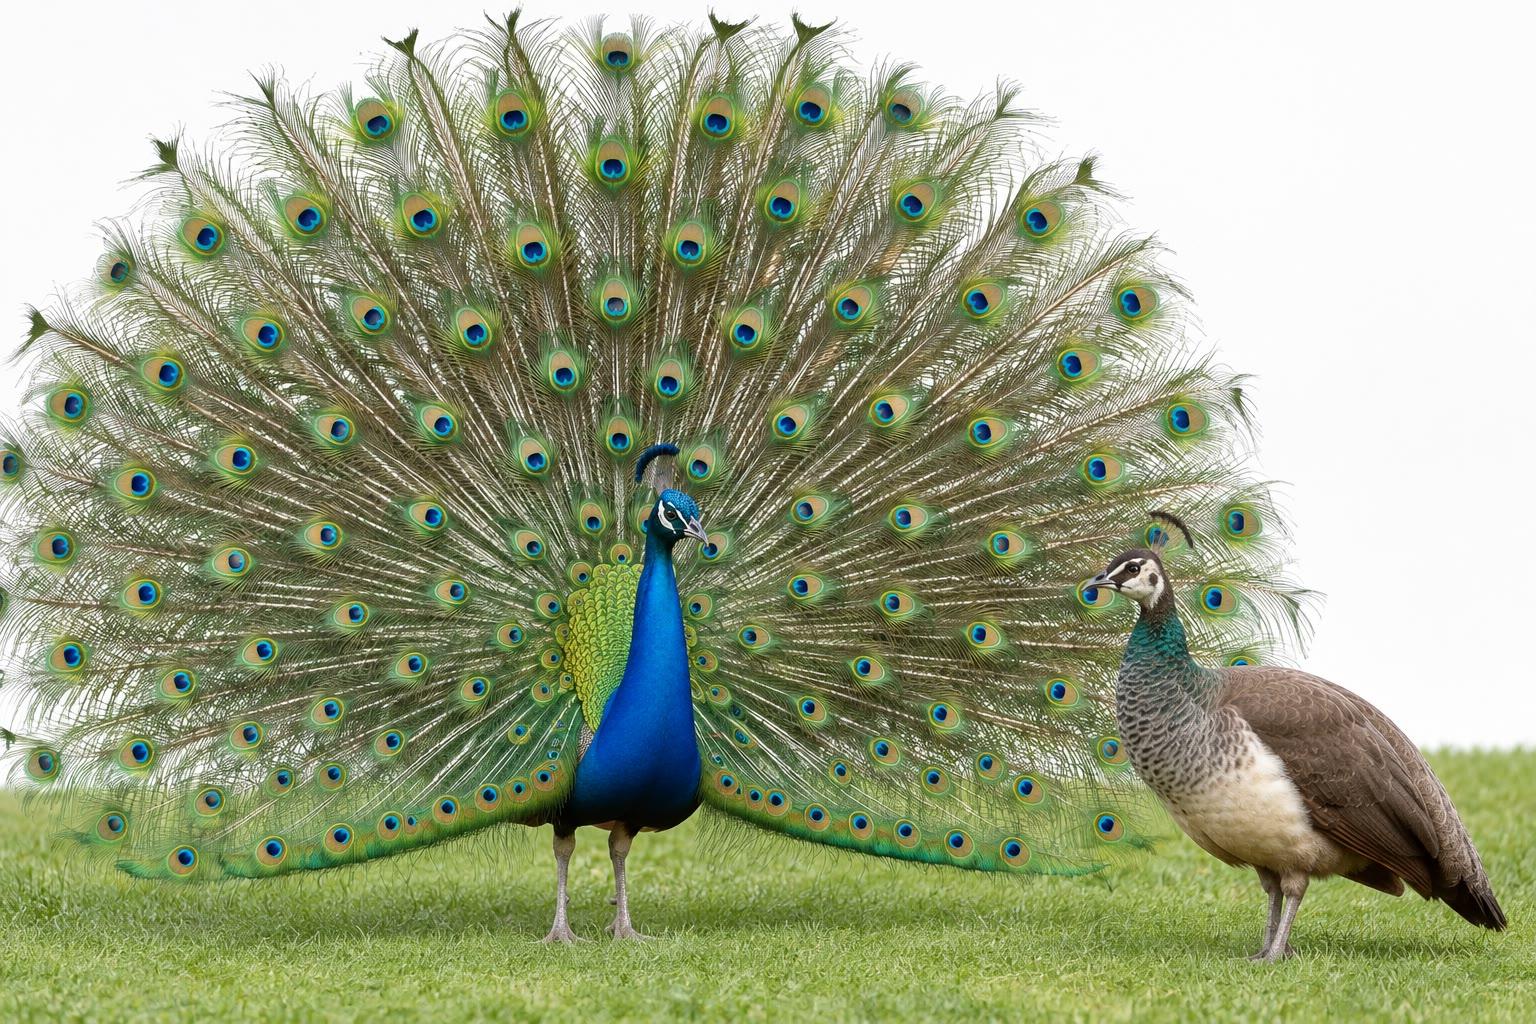
\includegraphics[width=0.46\linewidth]{images/book5/ai/b5-26-peacock-display.jpg}

{\small Izquierda: un suricata de guardia sobre un grupo de parientes
que forrajea. Derecha: un pavo real exhibiéndose ante una pava ---una
estructura que le cuesta a su portador comida y velocidad y no le
compra más que la atención de ella.}
\end{omfigure}

\section{Parejas y mensajes}

\begin{definition}[La selección sexual]\label{def:b3:behavioural-ecology:sexual-selection}
\index{selección sexual}\index{gradiente de Bateman}\index{selección desbocada}\index{principio del hándicap}\index{buenos genes}\index{conflicto sexual}
El segundo mecanismo de Darwin: la selección sobre rasgos que ganan
parejas y no supervivencia. Su raíz es la anisogamia ---la reproducción
de una hembra la limitan los huevos que puede fabricar y aprovisionar, y
la de un macho, las hembras a las que puede fecundar---, de modo que en
la mayoría de las especies la eficacia de un macho sube de forma
empinada con su número de apareamientos y la de una hembra apenas sube
(el \emph{gradiente de Bateman}); los machos compiten entonces por las
hembras y las hembras eligen entre los machos. La competencia da
cuernos, astas, colmillos, gran tamaño y los enfrentamientos de la
sección anterior. La elección da ornamentos, y tres explicaciones de por
qué los prefieren las hembras. La \emph{selección desbocada} de Fisher:
una preferencia por una cola algo más larga y la cola más larga se
extendieron juntas, y cada una volvió ventajosa a la otra hasta que el
coste de la cola en supervivencia equilibró su ganancia en
apareamientos. El \emph{hándicap} de Zahavi: un ornamento que solo un
macho sano puede permitirse desarrollar es una \omterm{prop:b3:behavioural-ecology:signals}{señal honesta} de su
condición, precisamente por ser costoso ---un pavo real con la cola
completa tiene, demostrablemente, menos parásitos. Los \emph{buenos
genes} y los \emph{beneficios directos}: la hembra gana a través de la
herencia de su descendencia o del territorio y el alimento que el macho
aporta. Los intereses de los dos sexos difieren, y el \emph{conflicto
sexual} ---sobre la frecuencia de apareamiento, sobre quién cuida de
las crías, sobre el destino del esperma de una pareja anterior--- es
una carrera de armamentos librada dentro de una especie: el líquido
seminal de los machos de la mosca del vinagre acorta la vida de la
hembra y eleva su puesta de huevos, y las hembras desarrollan
resistencia.
\end{definition}

\begin{proof}[Evidencia]
Andersson (1982) cortó y pegó las plumas de la cola de machos de
obispo colilargo en Kenia: los machos con la cola alargada hasta el
doble de su longitud natural atrajeron a sus territorios cuatro veces
más nidos nuevos que los machos con la cola acortada, mientras que los
controles, cuya cola se cortó y se volvió a pegar sin cambios, no se
vieron afectados ---una preferencia femenina por una cola más larga que
la de cualquier macho, la firma de una preferencia seleccionada más
allá del rasgo. Petrie (1994) halló que las pavas se apareaban con los
machos cuya cola llevaba más ocelos, y que los polluelos de esos machos
sobrevivían mejor en los bosques donde se los soltaba ---un beneficio de
\omterm{def:b3:behavioural-ecology:sexual-selection}{buenos genes} medido. Bateman (1948) contó apareamientos y descendencia
de moscas del vinagre portadoras de mutaciones marcadoras y halló el
gradiente que lleva su nombre: el éxito reproductivo de los machos
subía linealmente con los apareamientos, y el de las hembras se
estancaba tras el primero.
\end{proof}

\begin{proposition}[Las señales honestas]\label{prop:b3:behavioural-ecology:signals}
\index{comunicación}\index{señal honesta}\index{danza de la abeja}\index{señal referencial}
Una señal es un acto que cambia la conducta de un receptor y que
evolucionó para hacerlo; solo es estable si a las dos partes les
compensa, en promedio, enviarla y responder a ella. Allí donde ambas
tienen intereses comunes la señal puede ser barata y precisa: la
\emph{\omterm{prop:b3:behavioural-ecology:signals}{danza de la abeja}} de una forrajera (von Frisch, años cuarenta)
codifica la dirección de una fuente de alimento como el ángulo del
recorrido de meneo respecto de la vertical ---el ángulo de la fuente
respecto del sol--- y su distancia como la duración del recorrido, de
alrededor de un segundo por kilómetro, y las reclutadas vuelan hasta
unas decenas de metros del objetivo; los monos vervet dan llamadas de
alarma distintas para leopardos, águilas y serpientes, y quienes las
oyen responden de forma adecuada a cada llamada reproducida desde un
altavoz oculto ---señales \emph{referenciales}. Allí donde los intereses
chocan, una señal ha de ser costosa o imposible de falsificar para
seguir siendo honesta ---el bramido de un ciervo rojo, cuyo ritmo solo
puede sostener un macho en forma; el tamaño del croar de un sapo,
fijado por su cuerpo; los ornamentos del párrafo anterior--- o queda
explotada: las luciérnagas de un género imitan los destellos de las
hembras de otro para comerse a los machos que acuden, y los pollos de
cuco pujan más alto con sus reclamos que los propios del huésped. La
teoría de las señales predice así la forma de una señal a partir de la
relación entre las partes: barata e informativa entre parientes y
parejas cuyos intereses coinciden, cara y ritualizada entre rivales, y
una carrera de armamentos entre depredador y presa.
\end{proposition}
\admitted

\begin{omfigure}
\begin{tikzpicture}[every node/.style={font=\scriptsize}, >=stealth]
  % field view
  \node[above] at (0,3.2) {en el campo};
  \draw[->, thick, gray] (0,0) -- (0,2.6) node[above, font=\tiny] {hacia el sol};
  \fill[omDef!60] (0,0) circle (0.12); \node[below, font=\tiny] at (0,-0.2) {colmena};
  \draw[->, very thick, omThm] (0,0) -- ({2.4*sin(40)},{2.4*cos(40)}); \node[right, font=\tiny, omThm] at ({2.4*sin(40)},{2.4*cos(40)}) {alimento, \qty{1}{km}};
  \draw[omThm] (0,1.0) arc[start angle=90, end angle=50, radius=1.0]; \node[font=\tiny, omThm] at (0.55,1.25) {$40^{\circ}$};
  % comb view
  \begin{scope}[shift={(6.2,0)}]
    \node[above] at (0,3.2) {en el panal vertical};
    \draw[very thick, gray!60] (-1.8,-0.4) rectangle (1.8,3.0);
    \draw[->, thick, gray] (0,0) -- (0,2.6) node[above, font=\tiny] {arriba (= sol)};
    \draw[->, very thick, omThm] (0,0) -- ({1.6*sin(40)},{1.6*cos(40)}); \node[below, align=center, font=\tiny, omThm] at (0,-0.5) {recorrido de meneo: $40^{\circ}$ desde la vertical;\\duración $\approx \qty{1}{s}$ por km};
    \draw[omThm, dashed] ({1.6*sin(40)},{1.6*cos(40)}) .. controls (1.3,0.4) and (0.5,-0.3) .. (0,0);
    \draw[omThm, dashed] ({1.6*sin(40)},{1.6*cos(40)}) .. controls (-0.2,1.2) and (-0.6,0.3) .. (0,0);
    \draw[omThm] (0,0.8) arc[start angle=90, end angle=50, radius=0.8]; \node[font=\tiny, omThm] at (0.45,1.0) {$40^{\circ}$};
  \end{scope}
  \node[right, align=left] at (9.2,1.3) {un código simbólico: la gravedad\\representa al sol, y el tiempo\\a la distancia; las reclutadas llegan\\a unas decenas de metros};
\end{tikzpicture}

{\small La \omterm{prop:b3:behavioural-ecology:signals}{danza de la abeja}. El ángulo del recorrido respecto de la
vertical es el ángulo del alimento respecto del sol; la longitud del
recorrido es la distancia. Una señal tan barata y tan precisa es
posible porque la danzante y su público son hermanas con el mismo
interés.}
\end{omfigure}

\begin{omfigure}
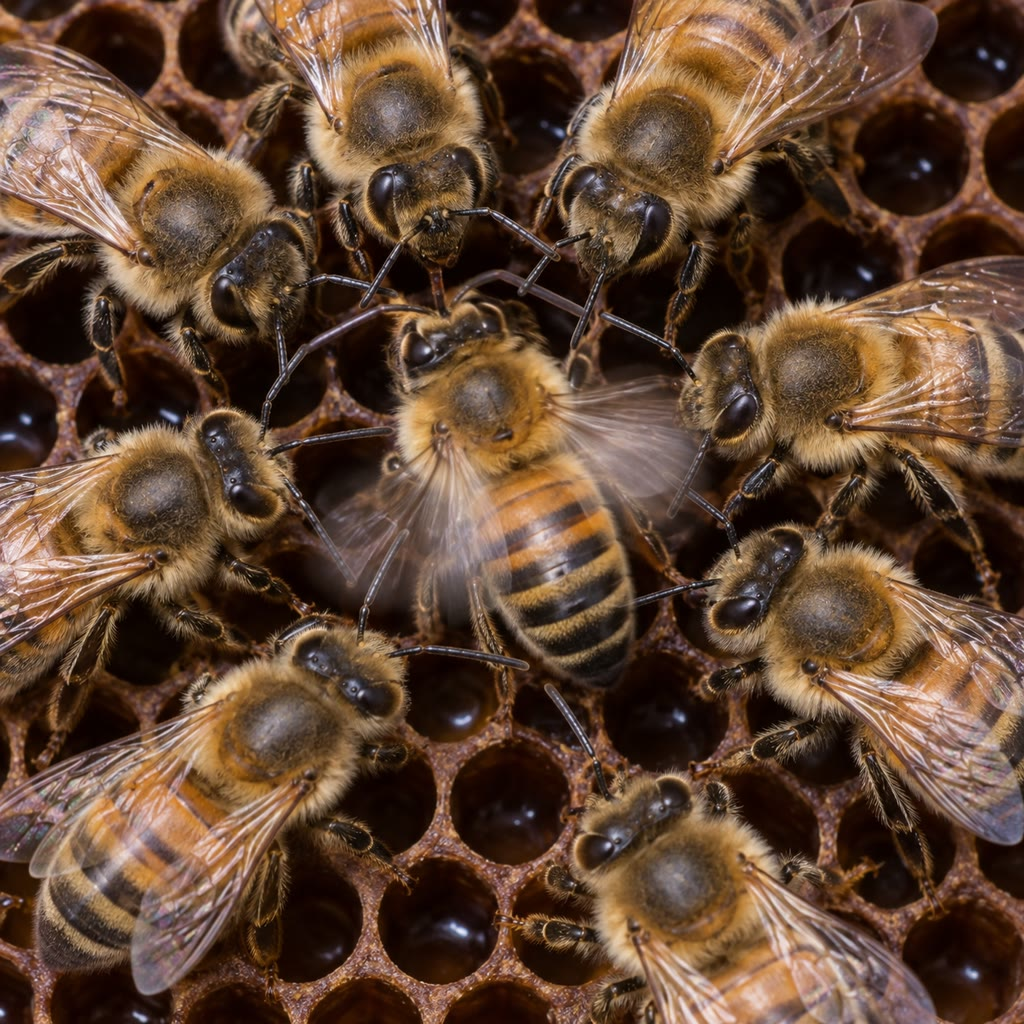
\includegraphics[width=0.4\linewidth]{images/book5/ai/b5-26-bee-dance.jpg}

{\small Una forrajera que baila sobre el panal, rodeada de obreras que
leen el ángulo y el tempo de su recorrido.}
\end{omfigure}

\begin{remark}[Por qué los animales parecen calcular]\label{rem:b3:behavioural-ecology:remark}
El carbonero no deriva $g(t)/(\tau + t)$, el suricata no calcula $r$ y
la pava jamás ha oído hablar de un hándicap. Cada uno lleva reglas
---márchate cuando las capturas se frenen, llama cuando el grupo sea
familia, prefiere al más brillante--- que la selección ha modelado
porque los animales que las seguían dejaron más descendientes; la
matemática es nuestra, una manera de preguntar qué han de conseguir las
reglas para que eso sea así, y de predecir la conducta en situaciones
que los animales no han encontrado nunca. Cuando las predicciones
fallan ---el carbonero se queda demasiado, el coste del centinela es
menor de lo supuesto---, el fallo es informativo: una moneda estaba mal
elegida, se pasó por alto una restricción, se contó mal a un pariente.
La materia es una conversación de décadas entre un cuaderno de campo y
una línea de álgebra, y las cuatro preguntas que planteó Tinbergen
siguen siendo el marco de ambos.
\end{remark}

\section{Ejercicios}

\begin{exercise}[$\star$]\label{exo:b3:behavioural-ecology:1}
Enúnciense las \omterm{def:b3:behavioural-ecology:tinbergen}{cuatro preguntas de Tinbergen} y respóndase a cada una,
en una frase, para la \omterm{prop:b3:behavioural-ecology:signals}{danza de la abeja}.
\end{exercise}

\begin{exercise}[$\star$]\label{exo:b3:behavioural-ecology:2}
¿Qué son una \omterm{def:b3:behavioural-ecology:tinbergen}{pauta fija de acción} y un \omterm{def:b3:behavioural-ecology:tinbergen}{estímulo señal}? Dense dos
ejemplos y explíquese qué mostró el palo ``supranormal'' con tres
bandas rojas.
\end{exercise}

\begin{exercise}[$\star$]\label{exo:b3:behavioural-ecology:3}
Con palabras, ¿qué dice el \omterm{thm:b3:behavioural-ecology:mvt}{teorema del valor marginal}, y qué predice
sobre el uso de los rodales cuando el tiempo de viaje se duplica?
\end{exercise}

\begin{exercise}[$\star$]\label{exo:b3:behavioural-ecology:4}
Defínase una EEE. ¿Por qué no lo es una población de Palomas puras, y
por qué la mezcla Halcón--Paloma cuesta a todos?
\end{exercise}

\begin{exercise}[$\star\star$]\label{exo:b3:behavioural-ecology:5}
Halcón--Paloma con $V = 6$ y $C = 10$: calcúlense $p^{*}$, el pago de
cada estrategia en la EEE y el pago que tendría una población de solo
Palomas. Repítase para $V = 12$ y $C = 10$.
\end{exercise}

\begin{exercise}[$\star\star$]\label{exo:b3:behavioural-ecology:6}
Una función de ganancia $g(t) = A(1 - \mathrm{e}^{-t/T_{0}})$ con $T_{0} =
\qty{2}{min}$. Hállense $t^{*}$ para $\tau = 2$ y $\tau = 8$ minutos
(úsense los valores del capítulo), la fracción de cada rodal consumida
y el ritmo a largo plazo $R$ como fracción de $A$ por minuto.
\end{exercise}

\begin{exercise}[$\star\star$]\label{exo:b3:behavioural-ecology:7}
Calcúlese $r$ entre: medio hermanos; abuelo y nieto; primos hermanos;
una obrera haplodiploide y su hermano; y una reina haplodiploide y su
hijo. Explíquense los dos últimos.
\end{exercise}

\begin{exercise}[$\star\star$]\label{exo:b3:behavioural-ecology:8}
Una llamada de alarma le cuesta a quien la da un \qty{2}{\%} de
probabilidad de muerte y libra a cada uno de $n$ parientes cercanos de
un \qty{1}{\%}. ¿Para qué $n$ favorece la \omterm{thm:b3:behavioural-ecology:hamilton}{regla de Hamilton} llamar si
los parientes son hermanos completos? ¿Y si son sobrinos? ¿Y si no hay
parentesco?
\end{exercise}

\begin{exercise}[$\star\star$]\label{exo:b3:behavioural-ecology:9}
La cola de un obispo colilargo mide \qty{50}{cm}; alargada a
\qty{75}{cm} atrae el doble de nidos, y acortada a \qty{25}{cm}, la
mitad. Si la supervivencia cae un \qty{20}{\%} por cada \qty{25}{cm}
añadidos, ¿qué cola maximiza el producto de apareamientos y
supervivencia, y por qué podría ser la cola natural más corta que esa?
\end{exercise}

\begin{exercise}[$\star\star\star$]\label{exo:b3:behavioural-ecology:10}
Añádase una tercera estrategia, Represalia, que exhibe como una Paloma
pero responde peleando si la atacan. Escríbanse sus pagos frente a
Halcón, Paloma y ella misma (frente a Halcón pelea: $(V - C)/2$; frente
a Paloma y a Represalia reparte: $V/2$). Muéstrese que una población de
Represalias no puede ser invadida por Halcones cuando $V < C$, y
discútase si las Palomas pueden colarse por deriva.
\end{exercise}

\begin{exercise}[$\star\star\star$]\label{exo:b3:behavioural-ecology:11}
En una guerra de desgaste, cada contendiente persiste durante un tiempo
extraído de una distribución; la EEE es exponencial con media
$V/$(coste por unidad de tiempo). Explíquese por qué un tiempo de
persistencia fijo no puede ser una EEE, y por qué una distribución
exponencial hace que la persistencia futura esperada de un oponente que
sigue exhibiéndose sea independiente de cuánto lleve ya exhibiéndose.
\end{exercise}

\begin{exercise}[$\star\star\star$]\label{exo:b3:behavioural-ecology:12}
El razonamiento de Hamilton sobre la haplodiploidía predice que las
obreras deberían preferir criar hermanas ($r = 3/4$) antes que hermanos
($r = 1/4$), mientras que la reina valora igual a hijos e hijas.
Predígase la proporción de sexos de los reproductores que debería
producir una colonia si la controlan las obreras y si la controla la
reina; dígase qué hallaron Trivers y Hare y qué le hace al razonamiento
una reina que se aparea con varios machos.
\end{exercise}

\section{Problema: la aritmética del centinela}

\begin{problem}[{Problema de fin de semana --- un día en un grupo de
suricatas hecho como ecología del comportamiento: los tiempos de rodal
del teorema del valor marginal, los enfrentamientos del juego
Halcón--Paloma y su EEE, la contabilidad de parentesco de la guardia y
de una colmena haplodiploide, y el coste de un ornamento, para terminar
en el tiempo de permanencia en el rodal, la frecuencia de Halcones y el
umbral de Hamilton del centinela}]
\label{pb:b3:behavioural-ecology:1}
Datos: rodales de forrajeo con $g(t) = A(1 - \mathrm{e}^{-t/T_{0}})$, $T_{0}
= \qty{3}{min}$, $A = \qty{60}{kJ}$; viaje entre rodales $\tau =
\qty{3}{min}$ (hábitat denso) o \qty{12}{min} (disperso).
Enfrentamientos por una madriguera: $V = 10$, $C = 30$ (unidades de
eficacia). Centinela: una hora de guardia le cuesta $c = 0.03$
equivalentes-descendiente (alimentación perdida, exposición); reduce el
riesgo de depredación de cada compañero de grupo en un valor de
$b = 0.01$ equivalentes-descendiente cada uno; el grupo tiene $n$
miembros de parentesco medio $\bar r$. Colmena: una obrera puede criar
$k$ hermanas o $k$ hijas propias con el mismo esfuerzo. Ornamento: una
longitud de cola $L$ da apareamientos $m(L) = L/20$ y supervivencia
$s(L) = 1 - (L/100)^{2}$, con $L$ en cm.

\medskip
\noindent\textbf{Parte I --- Los rodales.}
\begin{enumerate}
  \item Escríbanse el ritmo a largo plazo $R(t)$ y la condición del
        valor marginal para esta $g$.
  \item Muéstrese que la condición se reduce a $(\tau + t)/T_{0} = \mathrm{e}^{t/T_{0}}
        - 1$, y resuélvase para $\tau = T_{0}$ (pruébese con
        $t = 1.15\,T_{0}$).
  \item Resuélvase para $\tau = 4T_{0}$ (pruébese con $t = 2.0\,T_{0}$).
  \item Para cada caso: tiempo de permanencia en minutos, energía por
        rodal, fracción del rodal consumida y ritmo $R$ en kJ/min.
  \item Una regla práctica: ``márchate tras \qty{5}{min} fijos''.
        Calcúlese $R$ para los dos hábitats y compárese con el óptimo.
        ¿Basta la regla?
  \item Otra regla: ``márchate cuando pasen \qty{20}{s} sin una
        captura''. Explíquese por qué esta regla del tiempo de espera
        aproxima el teorema, y en qué sentido falla cuando los rodales
        difieren en riqueza.
\end{enumerate}

\medskip
\noindent\textbf{Parte II --- Los enfrentamientos.}
\begin{enumerate}[resume]
  \item Escríbase la matriz de pagos y calcúlese $p^{*}$.
  \item Pago del Halcón y de la Paloma cuando $p = 0.1$, $p = p^{*}$ y $p =
        0.6$; ¿qué estrategia se extiende en cada caso?
  \item Pago en la EEE; compárese con el pago de todo Palomas. ¿Cuánto
        pierde la población por enfrentamiento a causa de la posibilidad
        de pelear?
  \item Una sequía eleva $V$ a $40$ (madrigueras escasas). ¿Nueva EEE?
        ¿Qué predice esto sobre las peleas en los años duros?
  \item Burgués: ``Halcón si residente, Paloma si intruso'', cada papel
        la mitad de las veces. Su pago frente a sí mismo es $V/2$ sin
        peleas. Muéstrese que los Halcones no pueden invadir una
        población de Burgueses cuando $V
        < C$, y explíquese el caso de la mariposa nesóbara.
  \item Explíquese en una frase por qué gobierna esta conducta la
        dependencia de la frecuencia y no un óptimo.
\end{enumerate}

\medskip
\noindent\textbf{Parte III --- Los parientes.}
\begin{enumerate}[resume]
  \item \omterm{thm:b3:behavioural-ecology:hamilton}{Regla de Hamilton} para el centinela: condición sobre $n\bar r$.
        ¿Para qué $n\bar r$ compensa la guardia?
  \item Un grupo de $n = 8$ hermanos completos ($\bar r = 1/2$): ¿le
        compensa? ¿Y un grupo de 8 animales sin parentesco? ¿Y uno de 8
        medio hermanos?
  \item El centinela está bien alimentado, de modo que su $c$ cae a
        $0.01$. ¿Umbral ahora? ¿Por qué predice esto que los centinelas
        sean los individuos bien alimentados?
  \item La colmena: valor en \omterm{thm:b3:behavioural-ecology:hamilton}{eficacia inclusiva} de $k$ hermanas frente a
        $k$ hijas. ¿Qué debería preferir una obrera, y en qué
        proporción?
  \item La reina se ha apareado con tres machos por igual: ¿parentesco
        medio de las obreras con sus hermanas? ¿Sobrevive la
        preferencia?
  \item Explíquese por qué la \omterm{thm:b3:behavioural-ecology:hamilton}{regla de Hamilton} no exige que el actor
        reconozca a sus parientes, y qué regla práctica podría usar en
        realidad una ardilla terrestre.
\end{enumerate}

\medskip
\noindent\textbf{Parte IV --- Los ornamentos.}
\begin{enumerate}[resume]
  \item Eficacia $W(L) = m(L)\,s(L)$. Calcúlese $W$ para $L = 20$, $40$,
        $60$ y $80$.
  \item Hállese analíticamente la $L$ que maximiza $W$, y $W$ en ese
        punto.
  \item El coste en supervivencia se empina hasta $s = 1 - (L/70)^{2}$
        (llega un depredador). ¿Nuevo óptimo? ¿En qué sentido, y por qué
        predice esto que la cola siga en su evolución a la depredación?
  \item El experimento de Andersson duplicó las colas hasta
        \qty{75}{cm} y duplicó los nidos. ¿Es la preferencia femenina
        por colas más largas ``más allá del óptimo'' compatible con la
        explicación de la \omterm{def:b3:behavioural-ecology:sexual-selection}{selección desbocada}, con la del hándicap o con
        ambas?
  \item ¿Por qué un ornamento barato no es una \omterm{prop:b3:behavioural-ecology:signals}{señal honesta}, y cómo lo
        convierte en una el coste de la pregunta~21?
  \item \omterm{def:b3:behavioural-ecology:sexual-selection}{Gradientes de Bateman}: los machos ganan $0.8$ descendientes por
        apareamiento adicional, y las hembras $0.1$. Explíquese en un
        párrafo cómo esta asimetría genera a la vez los enfrentamientos
        de la Parte~II y los ornamentos de la Parte~IV.
  \item Resúmase: $t^{*}$ en el hábitat denso (pregunta~4), $p^{*}$
        (pregunta~7) y el umbral $n\bar r$ del centinela (pregunta~13).
\end{enumerate}
\end{problem}
